\documentclass{article}\usepackage[]{graphicx}\usepackage[]{xcolor}
% maxwidth is the original width if it is less than linewidth
% otherwise use linewidth (to make sure the graphics do not exceed the margin)
\makeatletter
\def\maxwidth{ %
  \ifdim\Gin@nat@width>\linewidth
    \linewidth
  \else
    \Gin@nat@width
  \fi
}
\makeatother

\definecolor{fgcolor}{rgb}{0.345, 0.345, 0.345}
\newcommand{\hlnum}[1]{\textcolor[rgb]{0.686,0.059,0.569}{#1}}%
\newcommand{\hlstr}[1]{\textcolor[rgb]{0.192,0.494,0.8}{#1}}%
\newcommand{\hlcom}[1]{\textcolor[rgb]{0.678,0.584,0.686}{\textit{#1}}}%
\newcommand{\hlopt}[1]{\textcolor[rgb]{0,0,0}{#1}}%
\newcommand{\hlstd}[1]{\textcolor[rgb]{0.345,0.345,0.345}{#1}}%
\newcommand{\hlkwa}[1]{\textcolor[rgb]{0.161,0.373,0.58}{\textbf{#1}}}%
\newcommand{\hlkwb}[1]{\textcolor[rgb]{0.69,0.353,0.396}{#1}}%
\newcommand{\hlkwc}[1]{\textcolor[rgb]{0.333,0.667,0.333}{#1}}%
\newcommand{\hlkwd}[1]{\textcolor[rgb]{0.737,0.353,0.396}{\textbf{#1}}}%
\let\hlipl\hlkwb

\usepackage{framed}
\makeatletter
\newenvironment{kframe}{%
 \def\at@end@of@kframe{}%
 \ifinner\ifhmode%
  \def\at@end@of@kframe{\end{minipage}}%
  \begin{minipage}{\columnwidth}%
 \fi\fi%
 \def\FrameCommand##1{\hskip\@totalleftmargin \hskip-\fboxsep
 \colorbox{shadecolor}{##1}\hskip-\fboxsep
     % There is no \\@totalrightmargin, so:
     \hskip-\linewidth \hskip-\@totalleftmargin \hskip\columnwidth}%
 \MakeFramed {\advance\hsize-\width
   \@totalleftmargin\z@ \linewidth\hsize
   \@setminipage}}%
 {\par\unskip\endMakeFramed%
 \at@end@of@kframe}
\makeatother

\definecolor{shadecolor}{rgb}{.97, .97, .97}
\definecolor{messagecolor}{rgb}{0, 0, 0}
\definecolor{warningcolor}{rgb}{1, 0, 1}
\definecolor{errorcolor}{rgb}{1, 0, 0}
\newenvironment{knitrout}{}{} % an empty environment to be redefined in TeX

\usepackage{alltt}
\usepackage[utf8]{inputenc}
\usepackage{amsfonts}
\usepackage{tgpagella}
\usepackage{graphicx} % Required for inserting images
\usepackage{polski}
\renewcommand*{\figurename}{Rysunek}
\usepackage{nicefrac, xfrac}
\usepackage[margin=1in]{geometry}
\usepackage{hyperref}
\usepackage{xcolor}
\usepackage{amssymb}
\usepackage[bottom]{footmisc}
\usepackage{float}
\IfFileExists{upquote.sty}{\usepackage{upquote}}{}
\begin{document}

\begin{knitrout}
\definecolor{shadecolor}{rgb}{0.969, 0.969, 0.969}\color{fgcolor}\begin{kframe}
\begin{alltt}
\hlkwd{library}\hlstd{(}\hlstr{"RMariaDB"}\hlstd{)}
\hlkwd{library}\hlstd{(tidyverse)}
\hlkwd{library}\hlstd{(ggplot2)}
\hlkwd{library}\hlstd{(eeptools)}
\hlkwd{library}\hlstd{(scales)}

\hlstd{con} \hlkwb{<-} \hlkwd{dbConnect}\hlstd{(RMariaDB}\hlopt{::}\hlkwd{MariaDB}\hlstd{(),}
                 \hlkwc{dbname} \hlstd{=} \hlstr{"team07"}\hlstd{,}
                 \hlkwc{username} \hlstd{=} \hlstr{"team07"}\hlstd{,}
                 \hlkwc{password} \hlstd{=} \hlstr{"te@m24ot"}\hlstd{,}
                 \hlkwc{host} \hlstd{=} \hlstr{"giniewicz.it"}\hlstd{)}
\hlstd{query} \hlkwb{<-} \hlstr{"SELECT * FROM klienci"}
\end{alltt}
\end{kframe}
\end{knitrout}

\section{Odsetek naprawianych marek pojazdów}
%Odsetek naprawianych marek pojazdów.

Przeprowadzono analizę, aby sprawdzić jakich marek pojazdy najczęściej pojawiają się w warsztacie do naprawy. Przyjęto, że każdy samochód lub motor jest liczony tylko raz, nawet jeżeli był kilkukrotnie naprawiany.

\begin{knitrout}
\definecolor{shadecolor}{rgb}{0.969, 0.969, 0.969}\color{fgcolor}\begin{kframe}
\begin{alltt}
\hlstd{query} \hlkwb{<-} \hlstr{"SELECT DISTINCT marka,
ROUND(100*count(marka)/SUM(COUNT(DISTINCT id_samochodu)) OVER (), 2) as procent
FROM usługi JOIN samochody
ON usługi.id_samochodu = samochody.id
GROUP BY marka ORDER BY count(marka) DESC"}

\hlstd{df} \hlkwb{<-} \hlkwd{dbGetQuery}\hlstd{(con, query)}
\hlstd{df[,}\hlnum{2}\hlstd{]} \hlkwb{<-} \hlkwd{as.numeric}\hlstd{(df[,}\hlnum{2}\hlstd{])}

\hlstd{minimalne} \hlkwb{<-} \hlstd{df} \hlopt \hlkwd{filter}\hlstd{(procent} \hlopt{==} \hlkwd{min}\hlstd{(procent))}
\hlstd{maksymalne} \hlkwb{<-} \hlstd{df} \hlopt \hlkwd{filter}\hlstd{(procent} \hlopt{==} \hlkwd{max}\hlstd{(procent))}

\hlstd{minimalne_tekst} \hlkwb{<-} \hlkwd{if_else}\hlstd{(}\hlkwd{length}\hlstd{(minimalne[,}\hlnum{1}\hlstd{])}\hlopt{>}\hlnum{1}\hlstd{,} \hlkwd{paste}\hlstd{(}\hlkwd{paste0}\hlstd{(minimalne[,}\hlnum{1}\hlstd{][}\hlnum{2}\hlopt{:}\hlkwd{length}\hlstd{(minimalne[,}\hlnum{1}\hlstd{])],} \hlkwc{collapse} \hlstd{=} \hlstr{", "}\hlstd{),} \hlstr{" i "}\hlstd{,minimalne[,}\hlnum{1}\hlstd{][}\hlnum{1}\hlstd{],} \hlkwc{sep}\hlstd{=}\hlstr{""}\hlstd{), minimalne[,}\hlnum{1}\hlstd{][}\hlnum{1}\hlstd{])}

\hlstd{maksymalne_tekst} \hlkwb{<-} \hlkwd{if_else}\hlstd{(}\hlkwd{length}\hlstd{(maksymalne[,}\hlnum{1}\hlstd{])}\hlopt{>}\hlnum{1}\hlstd{,} \hlkwd{paste}\hlstd{(}\hlkwd{paste0}\hlstd{(maksymalne[,}\hlnum{1}\hlstd{][}\hlnum{2}\hlopt{:}\hlkwd{length}\hlstd{(maksymalne[,}\hlnum{1}\hlstd{])],} \hlkwc{collapse} \hlstd{=} \hlstr{", "}\hlstd{),} \hlstr{" i "}\hlstd{,maksymalne[,}\hlnum{1}\hlstd{][}\hlnum{1}\hlstd{],} \hlkwc{sep}\hlstd{=}\hlstr{""}\hlstd{), maksymalne[,}\hlnum{1}\hlstd{][}\hlnum{1}\hlstd{])}

\hlstd{ranking} \hlkwb{<-} \hlkwd{paste0}\hlstd{(}\hlkwd{seq_len}\hlstd{(}\hlkwd{nrow}\hlstd{(df)),} \hlstr{". "}\hlstd{, df}\hlopt{$}\hlstd{marka,} \hlstr{": "}\hlstd{,} \hlkwd{paste}\hlstd{(df}\hlopt{$}\hlstd{procent,}\hlstr{"%"}\hlstd{,} \hlkwc{sep}\hlstd{=}\hlstr{""}\hlstd{),} \hlkwc{collapse} \hlstd{=} \hlstr{"\textbackslash{}n"}\hlstd{)}
\end{alltt}
\end{kframe}
\end{knitrout}

Można przedstawić procentowy udział marek pojazdów klientów salonu, zaczynając od najczęściej się pojawiającej:

\begin{verbatim}
1. Volkswagen: 14.22%
2. Opel: 11.61%
3. Ford: 8.77%
4. Renault: 6.16%
5. Audi: 6.16%
6. Hyundai: 4.98%
7. Skoda: 4.98%
8. Fiat: 4.74%
9. Bajaj: 4.27%
10. Mercedes-Benz: 3.79%
11. SEAT: 3.08%
12. BMW: 3.08%
13. Citroen: 3.08%
14. Honda: 2.61%
15. Suzuki: 2.37%
16. Kia: 2.37%
17. Nissan: 2.13%
18. Peugeot: 2.13%
19. Mazda: 1.9%
20. Yamaha: 1.66%
21. TVS: 1.42%
22. Hero: 1.42%
23. Toyota: 1.42%
24. Volvo: 1.18%
25. Mitsubishi: 0.95%
26. Dacia: 0.71%
27. Porsche: 0.71%
28. Royal: 0.47%
29. Chevrolet: 0.24%
30. Mahindra: 0.24%
31. Jaguar: 0.24%
32. SsangYong: 0.24%
33. MINI: 0.24%
34. Dodge: 0.24%
35. Vespa: 0.24%
36. Microcar: 0.24%
37. Jeep: 0.24%
\end{verbatim}

{\color{red} PROCENTY ZNAK}

Jak widać, najpopularniejsze są pojazdy marki Volkswagen. Pojazdy tej marki stanowią 14.22 wszystkich. \\

Najmniej popularne są marki Mahindra, Jaguar, SsangYong, MINI, Dodge, Vespa, Microcar, Jeep i Chevrolet. Każdą z nich reprezentowało 0.24 pojazdów, które się pojawiły w warsztacie.

Sprawdzono także, jak prezentowałyby się rozkład marek, gdyby brano pod uwagę jedynie samochody

\begin{knitrout}
\definecolor{shadecolor}{rgb}{0.969, 0.969, 0.969}\color{fgcolor}\begin{kframe}
\begin{alltt}
\hlstd{query} \hlkwb{<-} \hlstr{"SELECT DISTINCT marka,
ROUND(100*count(marka)/SUM(COUNT(DISTINCT id_samochodu)) OVER (), 2) as procent
FROM usługi JOIN (SELECT id, marka FROM samochody WHERE liczba_kół='4') as samochód
ON usługi.id_samochodu = samochód.id 
GROUP BY marka ORDER BY count(marka) DESC"}

\hlstd{df} \hlkwb{<-} \hlkwd{dbGetQuery}\hlstd{(con, query)}
\hlstd{df[,}\hlnum{2}\hlstd{]} \hlkwb{<-} \hlkwd{as.numeric}\hlstd{(df[,}\hlnum{2}\hlstd{])}

\hlstd{minimalne} \hlkwb{<-} \hlstd{df} \hlopt \hlkwd{filter}\hlstd{(procent} \hlopt{==} \hlkwd{min}\hlstd{(procent))}
\hlstd{maksymalne} \hlkwb{<-} \hlstd{df} \hlopt \hlkwd{filter}\hlstd{(procent} \hlopt{==} \hlkwd{max}\hlstd{(procent))}

\hlstd{minimalne_tekst} \hlkwb{<-} \hlkwd{if_else}\hlstd{(}\hlkwd{length}\hlstd{(minimalne[,}\hlnum{1}\hlstd{])}\hlopt{>}\hlnum{1}\hlstd{,} \hlkwd{paste}\hlstd{(}\hlkwd{paste0}\hlstd{(minimalne[,}\hlnum{1}\hlstd{][}\hlnum{2}\hlopt{:}\hlkwd{length}\hlstd{(minimalne[,}\hlnum{1}\hlstd{])],} \hlkwc{collapse} \hlstd{=} \hlstr{", "}\hlstd{),} \hlstr{" i "}\hlstd{,minimalne[,}\hlnum{1}\hlstd{][}\hlnum{1}\hlstd{],} \hlkwc{sep}\hlstd{=}\hlstr{""}\hlstd{), minimalne[,}\hlnum{1}\hlstd{][}\hlnum{1}\hlstd{])}

\hlstd{maksymalne_tekst} \hlkwb{<-} \hlkwd{if_else}\hlstd{(}\hlkwd{length}\hlstd{(maksymalne[,}\hlnum{1}\hlstd{])}\hlopt{>}\hlnum{1}\hlstd{,} \hlkwd{paste}\hlstd{(}\hlkwd{paste0}\hlstd{(maksymalne[,}\hlnum{1}\hlstd{][}\hlnum{2}\hlopt{:}\hlkwd{length}\hlstd{(maksymalne[,}\hlnum{1}\hlstd{])],} \hlkwc{collapse} \hlstd{=} \hlstr{", "}\hlstd{),} \hlstr{" i "}\hlstd{,maksymalne[,}\hlnum{1}\hlstd{][}\hlnum{1}\hlstd{],} \hlkwc{sep}\hlstd{=}\hlstr{""}\hlstd{), maksymalne[,}\hlnum{1}\hlstd{][}\hlnum{1}\hlstd{])}

\hlstd{df[,}\hlnum{2}\hlstd{]} \hlkwb{<-} \hlkwd{paste}\hlstd{(df[,}\hlnum{2}\hlstd{],}\hlstr{"%"}\hlstd{,} \hlkwc{sep}\hlstd{=}\hlstr{""}\hlstd{)}
\hlstd{ranking} \hlkwb{<-} \hlkwd{paste0}\hlstd{(}\hlkwd{seq_len}\hlstd{(}\hlkwd{nrow}\hlstd{(df)),} \hlstr{". "}\hlstd{, df}\hlopt{$}\hlstd{marka,} \hlstr{": "}\hlstd{, df}\hlopt{$}\hlstd{procent,} \hlkwc{collapse} \hlstd{=} \hlstr{"\textbackslash{}n"}\hlstd{)}
\end{alltt}
\end{kframe}
\end{knitrout}

Można przedstawić ranking marek, zaczynając od najczęściej się pojawiającej:

\begin{verbatim}
1. Volkswagen: 16.13%
2. Opel: 13.17%
3. Ford: 9.95%
4. Audi: 6.99%
5. Renault: 6.99%
6. Skoda: 5.65%
7. Hyundai: 5.65%
8. Fiat: 5.38%
9. Mercedes-Benz: 4.3%
10. Citroen: 3.49%
11. BMW: 3.49%
12. SEAT: 3.49%
13. Kia: 2.69%
14. Peugeot: 2.42%
15. Nissan: 2.42%
16. Mazda: 2.15%
17. Suzuki: 1.88%
18. Toyota: 1.61%
19. Volvo: 1.34%
20. Mitsubishi: 1.08%
21. Dacia: 0.81%
22. Porsche: 0.81%
23. Honda: 0.81%
24. SsangYong: 0.27%
25. Microcar: 0.27%
26. Jaguar: 0.27%
27. Dodge: 0.27%
28. Chevrolet: 0.27%
29. MINI: 0.27%
30. Jeep: 0.27%
\end{verbatim}

Wśród aut prym wiedzie Volkswagen, reprezentując  16.13 naprawianych samochodów. \\

Najmniej było samochodów marek Microcar, Jaguar, Dodge, Chevrolet, MINI, Jeep i SsangYong. Było ich 0.27 dla każdej. \\

Pozostały do sprawdzenia motory.

\begin{knitrout}
\definecolor{shadecolor}{rgb}{0.969, 0.969, 0.969}\color{fgcolor}\begin{kframe}
\begin{alltt}
\hlstd{query} \hlkwb{<-} \hlstr{"SELECT DISTINCT marka,
ROUND(100*count(marka)/SUM(COUNT(DISTINCT id_samochodu)) OVER (), 2) as procent
FROM usługi JOIN (SELECT id, marka FROM samochody WHERE liczba_kół='2') as motor
ON usługi.id_samochodu = motor.id 
GROUP BY marka ORDER BY count(marka) DESC"}

\hlstd{df} \hlkwb{<-} \hlkwd{dbGetQuery}\hlstd{(con, query)}
\hlstd{df[,}\hlnum{2}\hlstd{]} \hlkwb{<-} \hlkwd{as.numeric}\hlstd{(df[,}\hlnum{2}\hlstd{])}

\hlstd{minimalne} \hlkwb{<-} \hlstd{df} \hlopt \hlkwd{filter}\hlstd{(procent} \hlopt{==} \hlkwd{min}\hlstd{(procent))}
\hlstd{maksymalne} \hlkwb{<-} \hlstd{df} \hlopt \hlkwd{filter}\hlstd{(procent} \hlopt{==} \hlkwd{max}\hlstd{(procent))}

\hlstd{minimalne_tekst} \hlkwb{<-} \hlkwd{if_else}\hlstd{(}\hlkwd{length}\hlstd{(minimalne[,}\hlnum{1}\hlstd{])}\hlopt{>}\hlnum{1}\hlstd{,} \hlkwd{paste}\hlstd{(}\hlkwd{paste0}\hlstd{(minimalne[,}\hlnum{1}\hlstd{][}\hlnum{2}\hlopt{:}\hlkwd{length}\hlstd{(minimalne[,}\hlnum{1}\hlstd{])],} \hlkwc{collapse} \hlstd{=} \hlstr{", "}\hlstd{),} \hlstr{" i "}\hlstd{,minimalne[,}\hlnum{1}\hlstd{][}\hlnum{1}\hlstd{],} \hlkwc{sep}\hlstd{=}\hlstr{""}\hlstd{), minimalne[,}\hlnum{1}\hlstd{][}\hlnum{1}\hlstd{])}

\hlstd{maksymalne_tekst} \hlkwb{<-} \hlkwd{if_else}\hlstd{(}\hlkwd{length}\hlstd{(maksymalne[,}\hlnum{1}\hlstd{])}\hlopt{>}\hlnum{1}\hlstd{,} \hlkwd{paste}\hlstd{(}\hlkwd{paste0}\hlstd{(maksymalne[,}\hlnum{1}\hlstd{][}\hlnum{2}\hlopt{:}\hlkwd{length}\hlstd{(maksymalne[,}\hlnum{1}\hlstd{])],} \hlkwc{collapse} \hlstd{=} \hlstr{", "}\hlstd{),} \hlstr{" i "}\hlstd{,maksymalne[,}\hlnum{1}\hlstd{][}\hlnum{1}\hlstd{],} \hlkwc{sep}\hlstd{=}\hlstr{""}\hlstd{), maksymalne[,}\hlnum{1}\hlstd{][}\hlnum{1}\hlstd{])}

\hlstd{df[,}\hlnum{2}\hlstd{]} \hlkwb{<-} \hlkwd{paste}\hlstd{(df[,}\hlnum{2}\hlstd{],}\hlstr{"%"}\hlstd{,} \hlkwc{sep}\hlstd{=}\hlstr{""}\hlstd{)}
\hlstd{ranking} \hlkwb{<-} \hlkwd{paste0}\hlstd{(}\hlkwd{seq_len}\hlstd{(}\hlkwd{nrow}\hlstd{(df)),} \hlstr{". "}\hlstd{, df}\hlopt{$}\hlstd{marka,} \hlstr{": "}\hlstd{, df}\hlopt{$}\hlstd{procent,} \hlkwc{collapse} \hlstd{=} \hlstr{"\textbackslash{}n"}\hlstd{)}
\end{alltt}
\end{kframe}
\end{knitrout}

Udział procentowy poszczególnych marek wśród nich prezentuje się następująco:

\begin{verbatim}
1. Bajaj: 36%
2. Honda: 16%
3. Yamaha: 14%
4. TVS: 12%
5. Hero: 12%
6. Suzuki: 6%
7. Royal: 4%
8. Vespa: 2%
9. Mahindra: 2%
\end{verbatim}

Wśród nich najczęściej naprawiano motory marki Bajaj. Pojazdy tej marki stanowią 36.00 wszystkich. \\

Najmniej popularnymi motorami są z kolei modele marek Mahindra i Vespa. W warsztacie było zaledwie 2.00 motorów,tej marki.


\section{Analiza bilansu}

\subsection{Analiza wydatków na zakup pojazdów}

\begin{knitrout}
\definecolor{shadecolor}{rgb}{0.969, 0.969, 0.969}\color{fgcolor}\begin{kframe}
\begin{alltt}
\hlstd{query} \hlkwb{<-} \hlstr{"SELECT CONCAT(DATE_FORMAT(data_zaksięgowania, '%Y-%m'), '-01')
AS data, SUM(cena) as suma
FROM zakup_samochodu GROUP BY data ORDER BY data"}

\hlstd{df} \hlkwb{<-} \hlkwd{dbGetQuery}\hlstd{(con, query)}
\hlstd{df[,}\hlnum{1}\hlstd{]} \hlkwb{<-} \hlkwd{as.Date}\hlstd{(df[,}\hlnum{1}\hlstd{])}
\hlstd{df[,}\hlnum{2}\hlstd{]} \hlkwb{<-} \hlkwd{as.numeric}\hlstd{(df[,}\hlnum{2}\hlstd{])}

\hlstd{wszystkie_daty} \hlkwb{<-} \hlkwd{expand.grid}\hlstd{(}\hlnum{1}\hlopt{:}\hlnum{12}\hlstd{,} \hlnum{2014}\hlopt{:}\hlnum{2017}\hlstd{) |>} \hlkwd{reframe}\hlstd{(}\hlkwc{data} \hlstd{=} \hlkwd{make_date}\hlstd{(Var2, Var1,} \hlnum{1}\hlstd{))}
\hlstd{df} \hlkwb{<-} \hlkwd{merge}\hlstd{(}\hlkwc{x}\hlstd{=df,} \hlkwc{y}\hlstd{=wszystkie_daty,} \hlkwc{by}\hlstd{=}\hlstr{"data"}\hlstd{,} \hlkwc{all.y}\hlstd{=T)}
\hlstd{df}\hlopt{$}\hlstd{suma[}\hlkwd{is.na}\hlstd{(df}\hlopt{$}\hlstd{suma)]} \hlkwb{<-} \hlnum{0}

\hlstd{df |>} \hlkwd{ggplot}\hlstd{(}\hlkwd{aes}\hlstd{(}\hlkwc{x}\hlstd{=data,} \hlkwc{y}\hlstd{=suma, ,} \hlkwc{fill}\hlstd{=}\hlkwd{format}\hlstd{(data,} \hlstr{"%m"}\hlstd{)))} \hlopt{+}
  \hlkwd{geom_bar}\hlstd{(}\hlkwc{stat} \hlstd{=} \hlstr{"identity"}\hlstd{)} \hlopt{+}
  \hlkwd{scale_fill_manual}\hlstd{(}\hlkwc{name}\hlstd{=}\hlstr{"Miesiąc"}\hlstd{,}\hlkwc{labels}\hlstd{=}\hlkwd{unique}\hlstd{(}\hlkwd{format}\hlstd{(df}\hlopt{$}\hlstd{data,} \hlstr{"%B"}\hlstd{)),} \hlkwc{values}\hlstd{=}\hlkwd{hue_pal}\hlstd{()(}\hlnum{12}\hlstd{))}
\end{alltt}
\end{kframe}
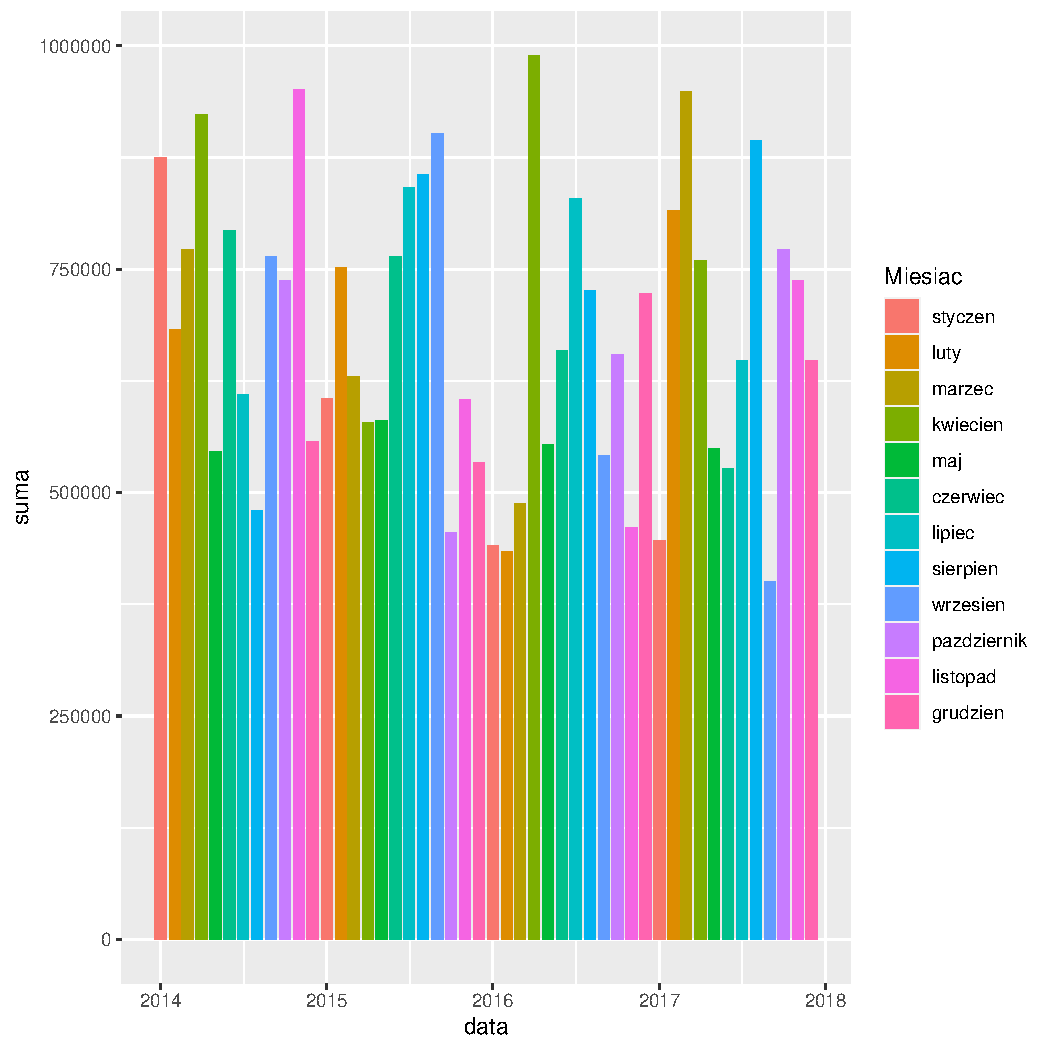
\includegraphics[width=\maxwidth]{figure/unnamed-chunk-5-1} 
\end{knitrout}


\subsection{Analiza wydatków na zakup części}

\begin{knitrout}
\definecolor{shadecolor}{rgb}{0.969, 0.969, 0.969}\color{fgcolor}\begin{kframe}
\begin{alltt}
\hlstd{query} \hlkwb{<-} \hlstr{"SELECT CONCAT(DATE_FORMAT(data_zaksięgowania, '%Y-%m'), '-01') as data,
SUM(użyte_części.cena*użyte_części.ilość) as suma
FROM usługi JOIN użyte_części
ON usługi.id = użyte_części.id_usługi
GROUP BY data ORDER BY data"}

\hlstd{df} \hlkwb{<-} \hlkwd{dbGetQuery}\hlstd{(con, query)}
\hlstd{df[,}\hlnum{1}\hlstd{]} \hlkwb{<-} \hlkwd{as.Date}\hlstd{(df[,}\hlnum{1}\hlstd{])}
\hlstd{df[,}\hlnum{2}\hlstd{]} \hlkwb{<-} \hlkwd{as.numeric}\hlstd{(df[,}\hlnum{2}\hlstd{])}

\hlstd{wszystkie_daty} \hlkwb{<-} \hlkwd{expand.grid}\hlstd{(}\hlnum{1}\hlopt{:}\hlnum{12}\hlstd{,} \hlnum{2014}\hlopt{:}\hlnum{2017}\hlstd{) |>} \hlkwd{reframe}\hlstd{(}\hlkwc{data} \hlstd{=} \hlkwd{make_date}\hlstd{(Var2, Var1,} \hlnum{1}\hlstd{))}
\hlstd{df} \hlkwb{<-} \hlkwd{merge}\hlstd{(}\hlkwc{x}\hlstd{=df,} \hlkwc{y}\hlstd{=wszystkie_daty,} \hlkwc{by}\hlstd{=}\hlstr{"data"}\hlstd{,} \hlkwc{all.y}\hlstd{=T)}
\hlstd{df}\hlopt{$}\hlstd{suma[}\hlkwd{is.na}\hlstd{(df}\hlopt{$}\hlstd{suma)]} \hlkwb{<-} \hlnum{0}

\hlstd{df |>} \hlkwd{ggplot}\hlstd{(}\hlkwd{aes}\hlstd{(}\hlkwc{x}\hlstd{=data,} \hlkwc{y}\hlstd{=suma, ,} \hlkwc{fill}\hlstd{=}\hlkwd{format}\hlstd{(data,} \hlstr{"%m"}\hlstd{)))} \hlopt{+}
  \hlkwd{geom_bar}\hlstd{(}\hlkwc{stat} \hlstd{=} \hlstr{"identity"}\hlstd{)} \hlopt{+}
  \hlkwd{scale_fill_manual}\hlstd{(}\hlkwc{name}\hlstd{=}\hlstr{"Miesiąc"}\hlstd{,}\hlkwc{labels}\hlstd{=}\hlkwd{unique}\hlstd{(}\hlkwd{format}\hlstd{(df}\hlopt{$}\hlstd{data,} \hlstr{"%B"}\hlstd{)),} \hlkwc{values}\hlstd{=}\hlkwd{hue_pal}\hlstd{()(}\hlnum{12}\hlstd{))}
\end{alltt}
\end{kframe}
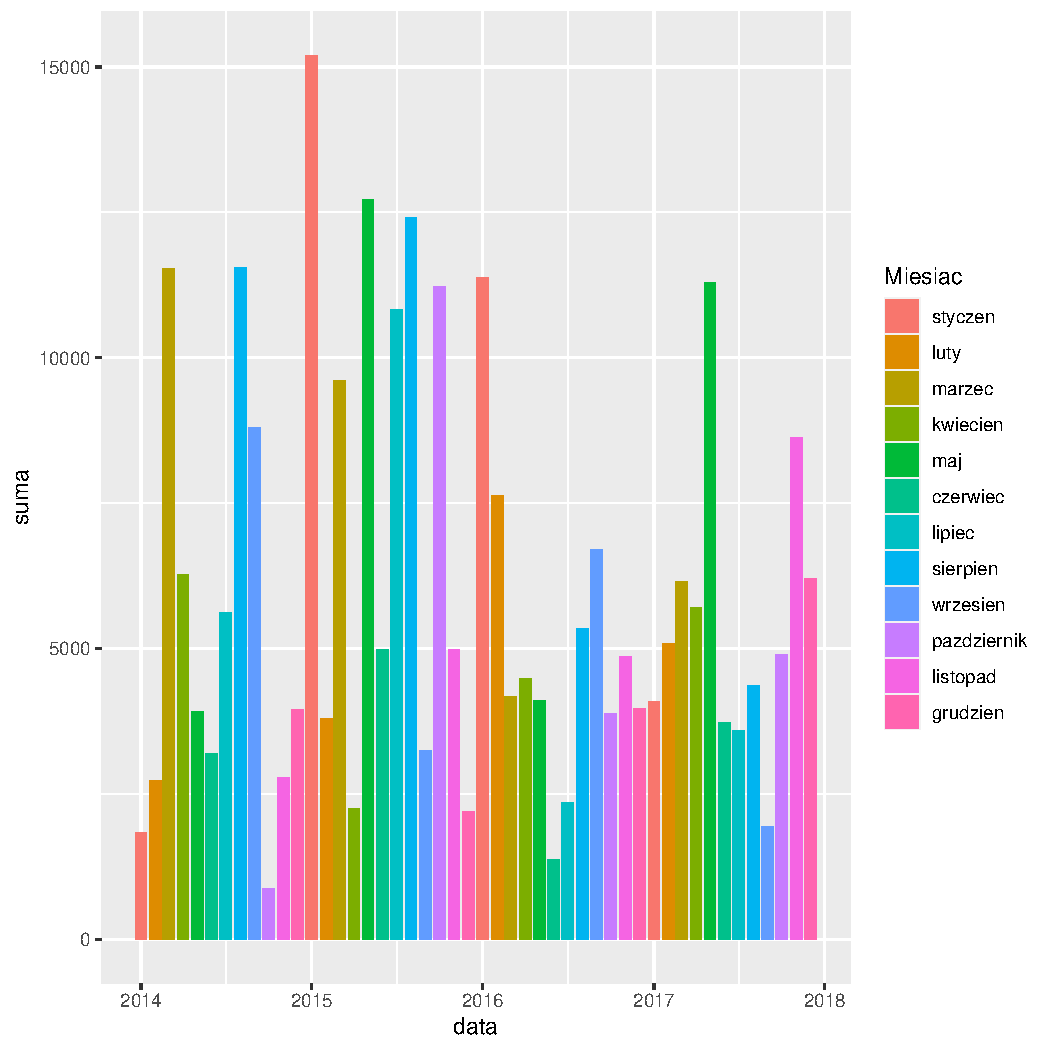
\includegraphics[width=\maxwidth]{figure/unnamed-chunk-6-1} 
\end{knitrout}

\subsection{Analiza przychodów z usług warsztatu}

\begin{knitrout}
\definecolor{shadecolor}{rgb}{0.969, 0.969, 0.969}\color{fgcolor}\begin{kframe}
\begin{alltt}
\hlstd{query} \hlkwb{<-} \hlstr{"SELECT CONCAT(DATE_FORMAT(data_zaksięgowania, '%Y-%m'), '-01') as data,
SUM(usługi.cena) - SUM(użyte_części.cena*użyte_części.ilość) as suma
FROM usługi JOIN użyte_części
ON usługi.id = użyte_części.id_usługi
GROUP BY data ORDER BY data"}

\hlstd{df} \hlkwb{<-} \hlkwd{dbGetQuery}\hlstd{(con, query)}
\hlstd{df[,}\hlnum{1}\hlstd{]} \hlkwb{<-} \hlkwd{as.Date}\hlstd{(df[,}\hlnum{1}\hlstd{])}
\hlstd{df[,}\hlnum{2}\hlstd{]} \hlkwb{<-} \hlkwd{as.numeric}\hlstd{(df[,}\hlnum{2}\hlstd{])}

\hlstd{wszystkie_daty} \hlkwb{<-} \hlkwd{expand.grid}\hlstd{(}\hlnum{1}\hlopt{:}\hlnum{12}\hlstd{,} \hlnum{2014}\hlopt{:}\hlnum{2017}\hlstd{) |>} \hlkwd{reframe}\hlstd{(}\hlkwc{data} \hlstd{=} \hlkwd{make_date}\hlstd{(Var2, Var1,} \hlnum{1}\hlstd{))}
\hlstd{df} \hlkwb{<-} \hlkwd{merge}\hlstd{(}\hlkwc{x}\hlstd{=df,} \hlkwc{y}\hlstd{=wszystkie_daty,} \hlkwc{by}\hlstd{=}\hlstr{"data"}\hlstd{,} \hlkwc{all.y}\hlstd{=T)}
\hlstd{df}\hlopt{$}\hlstd{suma[}\hlkwd{is.na}\hlstd{(df}\hlopt{$}\hlstd{suma)]} \hlkwb{<-} \hlnum{0}

\hlstd{df |>} \hlkwd{ggplot}\hlstd{(}\hlkwd{aes}\hlstd{(}\hlkwc{x}\hlstd{=data,} \hlkwc{y}\hlstd{=suma, ,} \hlkwc{fill}\hlstd{=}\hlkwd{format}\hlstd{(data,} \hlstr{"%m"}\hlstd{)))} \hlopt{+}
  \hlkwd{geom_bar}\hlstd{(}\hlkwc{stat} \hlstd{=} \hlstr{"identity"}\hlstd{)} \hlopt{+}
  \hlkwd{scale_fill_manual}\hlstd{(}\hlkwc{name}\hlstd{=}\hlstr{"Miesiąc"}\hlstd{,}\hlkwc{labels}\hlstd{=}\hlkwd{unique}\hlstd{(}\hlkwd{format}\hlstd{(df}\hlopt{$}\hlstd{data,} \hlstr{"%B"}\hlstd{)),} \hlkwc{values}\hlstd{=}\hlkwd{hue_pal}\hlstd{()(}\hlnum{12}\hlstd{))}
\end{alltt}
\end{kframe}
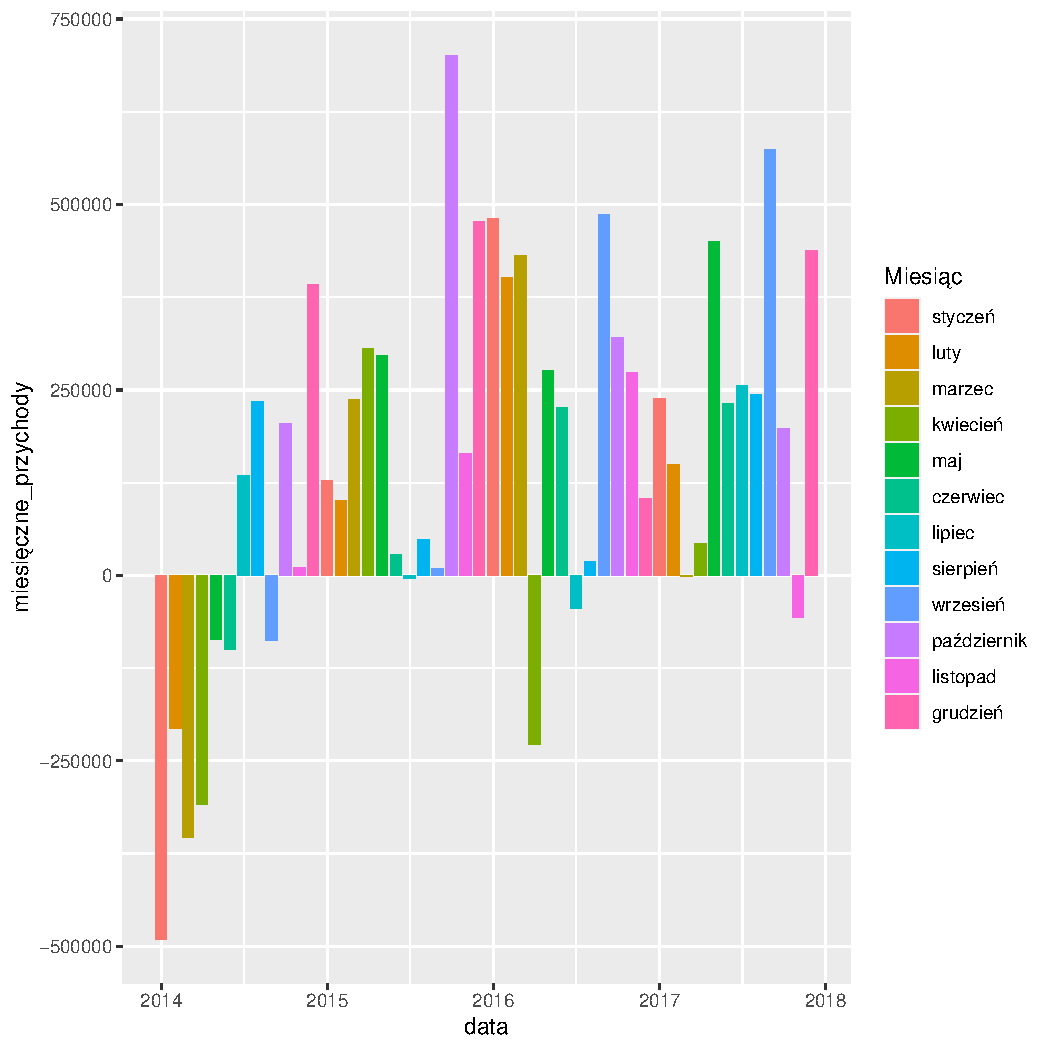
\includegraphics[width=\maxwidth]{figure/unnamed-chunk-7-1} 
\end{knitrout}

\subsection{Koszty wypłat dla pracowników}


\section{Kim są najlepszy mechanik i sprzedawca w warsztacie?}

Przez czas działania warsztatu „Pimp My Wheels” osoba zarządzająca warsztatem nie była skłonna do dawania podwyżek, jednak postanowiła zlecić informatykowi by przeanalizował bazę danych i znalazł pracowników, którzy zasługują na większe wynagrodzenie.


\begin{knitrout}
\definecolor{shadecolor}{rgb}{0.969, 0.969, 0.969}\color{fgcolor}\begin{kframe}
\begin{alltt}
\hlstd{query} \hlkwb{<-} \hlstr{"SELECT CONCAT(imię, ' ',nazwisko) as sprzedawca, SUM(sprzedaż_samochodu.cena) as suma,
COUNT(sprzedaż_samochodu.cena) as ile_sprzedanych, płaca, id_pracownika
FROM sprzedaż_samochodu
JOIN pracownicy ON sprzedaż_samochodu.id_pracownika=pracownicy.id
GROUP BY sprzedaż_samochodu.id_pracownika ORDER BY suma"}

\hlstd{df} \hlkwb{<-} \hlkwd{dbGetQuery}\hlstd{(con, query)}

\hlstd{najwiecej_zarobił} \hlkwb{<-} \hlstd{df} \hlopt \hlkwd{filter}\hlstd{(suma} \hlopt{==} \hlkwd{max}\hlstd{(suma))}
\hlstd{najwiecej_sprzedaży} \hlkwb{<-} \hlstd{df} \hlopt \hlkwd{filter}\hlstd{(ile_sprzedanych} \hlopt{==} \hlkwd{max}\hlstd{(ile_sprzedanych))}

\hlstd{średnia_płaca} \hlkwb{<-} \hlkwd{mean}\hlstd{(df}\hlopt{$}\hlstd{płaca)}
\hlstd{średnia_suma} \hlkwb{<-} \hlkwd{mean}\hlstd{(df}\hlopt{$}\hlstd{suma)}
\hlstd{średnia_ilość} \hlkwb{<-} \hlkwd{mean}\hlstd{(df}\hlopt{$}\hlstd{ile_sprzedanych)}

\hlstd{procent_suma_zarobił} \hlkwb{<-} \hlstd{(najwiecej_zarobił}\hlopt{$}\hlstd{suma} \hlopt{/} \hlstd{średnia_suma)} \hlopt{*} \hlnum{100}
\hlstd{procent_placa_zarobił} \hlkwb{<-} \hlstd{(najwiecej_zarobił}\hlopt{$}\hlstd{płaca} \hlopt{/} \hlstd{średnia_płaca)} \hlopt{*} \hlnum{100}

\hlstd{różnica_zarobił} \hlkwb{<-} \hlkwd{round}\hlstd{(procent_suma_zarobił}\hlopt{-}\hlstd{procent_placa_zarobił,}\hlnum{2}\hlstd{)}

\hlstd{procent_suma_sprzedaży} \hlkwb{<-} \hlstd{(najwiecej_sprzedaży}\hlopt{$}\hlstd{ile_sprzedanych} \hlopt{/} \hlstd{średnia_ilość)} \hlopt{*} \hlnum{100}
\hlstd{procent_placa_sprzedaży} \hlkwb{<-} \hlstd{(najwiecej_sprzedaży}\hlopt{$}\hlstd{płaca} \hlopt{/} \hlstd{średnia_płaca)} \hlopt{*} \hlnum{100}

\hlstd{różnica_sprzedaż} \hlkwb{<-} \hlkwd{round}\hlstd{(procent_suma_sprzedaży} \hlopt{-} \hlstd{procent_placa_sprzedaży,} \hlnum{2}\hlstd{)}

\hlkwa{if} \hlstd{(najwiecej_sprzedaży[,}\hlnum{5}\hlstd{]} \hlopt{==} \hlstd{najwiecej_zarobił[,}\hlnum{5}\hlstd{])\{ten_sam}\hlkwb{=}\hlkwd{c}\hlstd{(}\hlstr{"ponownie "}\hlstd{)\}} \hlkwa{else} \hlstd{\{ten_sam}\hlkwb{=}\hlkwd{rep}\hlstd{(}\hlstr{""}\hlstd{,} \hlnum{1}\hlstd{)\}}


\hlkwa{if} \hlstd{(}\hlkwd{length}\hlstd{(najwiecej_zarobił[,}\hlnum{1}\hlstd{])}\hlopt{>}\hlnum{1}\hlstd{)\{}
  \hlstd{tekst_sprzedaż1}\hlkwb{=}\hlkwd{paste}\hlstd{(}\hlstr{"Osoby, które sprzedały w firmie najwięcej pojazdów to "}\hlstd{,, najwiecej_zarobił[,}\hlnum{1}\hlstd{] ,}\hlstr{". Te osoby sprzedały"}\hlstd{)}
  \hlstd{\}} \hlkwa{else} \hlstd{\{ tekst_sprzedaż1}\hlkwb{=} \hlkwd{paste}\hlstd{(}\hlstr{"Osoba, która sprzedała w firmie najbardziej wartościowe pojazdy to "}\hlstd{, najwiecej_zarobił[,}\hlnum{1}\hlstd{],}
\hlstr{". Ta osoba zarobiła dla firmy "}\hlstd{,} \hlkwd{format}\hlstd{(}\hlkwd{round}\hlstd{(najwiecej_zarobił}\hlopt{$}\hlstd{suma,}\hlnum{2}\hlstd{),} \hlkwc{nsmall} \hlstd{=} \hlnum{2}\hlstd{),} \hlstr{" zł na sprzedaży pojazdów, co stanowi "}\hlstd{,} \hlkwd{format}\hlstd{(}\hlkwd{round}\hlstd{(procent_suma_zarobił,}\hlnum{2}\hlstd{),} \hlkwc{nsmall} \hlstd{=} \hlnum{2}\hlstd{),}
\hlstr{"\textbackslash{}\textbackslash{}% średniej kwoty zarobionej dla warsztatu przez cały okres pracy. W porównaniu, zarabiana przez tego pracownika kwota za godzinę pracy ("}\hlstd{,} \hlkwd{format}\hlstd{(}\hlkwd{round}\hlstd{(najwiecej_zarobił}\hlopt{$}\hlstd{płaca,}\hlnum{2}\hlstd{),} \hlkwc{nsmall} \hlstd{=} \hlnum{2}\hlstd{),} \hlstr{" zł) stanowi "}\hlstd{,} \hlkwd{format}\hlstd{(}\hlkwd{round}\hlstd{(procent_placa_zarobił,}\hlnum{2}\hlstd{),} \hlkwc{nsmall} \hlstd{=} \hlnum{2}\hlstd{),} \hlstr{" \textbackslash{}\textbackslash{}% średniej płacy sprzedawcy ("}\hlstd{,}
\hlkwd{format}\hlstd{(}\hlkwd{round}\hlstd{(średnia_płaca,}\hlnum{2}\hlstd{),} \hlkwc{nsmall} \hlstd{=} \hlnum{2}\hlstd{) ,} \hlstr{" zł). Różnica procentowa wynosi "}\hlstd{,}
\hlkwd{format}\hlstd{(}\hlkwd{abs}\hlstd{(różnica_zarobił),} \hlkwc{nsmall} \hlstd{=} \hlnum{2}\hlstd{),} \hlstr{"\textbackslash{}\textbackslash{}%"}\hlstd{,}
\hlkwd{if_else}\hlstd{(różnica_zarobił} \hlopt{<} \hlnum{0}  \hlstd{,} \hlstr{" na korzyść pracownika, czyli warsztat nie musi koniecznie zwiększać stawki godzinowej tego sprzedawcy."}\hlstd{,} \hlkwd{if_else}\hlstd{(różnica_zarobił} \hlopt{<} \hlnum{2}\hlstd{,} \hlstr{", czyli warsztat nie musi koniecznie zwiększać stawki godzinowej tego sprzedawcy, jako że różnica jest niewielka. Można jednak nad tym pomyśleć, by zachęcić pracownika do dalszej pracy i jeszcze lepszych wyników."}\hlstd{,} \hlkwd{if_else}\hlstd{(}
  \hlstd{różnica_zarobił} \hlopt{<} \hlnum{5}\hlstd{,} \hlstr{", czyli warsztat powinien rozważyć podwyżkę dla tego pracownika, by zachęcić go do dalszej pracy i jeszcze lepszych wyników."}\hlstd{,} \hlstr{", czyli warsztat zdecydowanie powinien rozważyć podwyżkę dla tego pracownika, by lepiej wyróżnić jego wpływ na dochody firmy."}\hlstd{))),} \hlkwc{sep}\hlstd{=}\hlstr{""}\hlstd{)}
  \hlstd{\}}

\hlkwa{if} \hlstd{(}\hlkwd{length}\hlstd{(najwiecej_zarobił[,}\hlnum{1}\hlstd{])}\hlopt{>}\hlnum{1}\hlstd{)\{}
  \hlstd{tekst_sprzedaż2}\hlkwb{=}\hlkwd{paste}\hlstd{(}\hlstr{"Osoby, które sprzedały w firmie najwięcej pojazdów to "}\hlstd{, najwiecej_sprzedaży[,}\hlnum{1}\hlstd{] ,}\hlstr{". Te osoby sprzedały"}\hlstd{)}
  \hlstd{\}} \hlkwa{else} \hlstd{\{}
\hlstd{tekst_sprzedaż2} \hlkwb{=} \hlkwd{paste}\hlstd{(}\hlstr{"Pracownik, który sprzedał najwięcej pojazdów to "}\hlstd{, ten_sam[}\hlnum{1}\hlstd{], najwiecej_sprzedaży[,}\hlnum{1}\hlstd{],}
\hlstr{". Ta osoba sprzedała aż "}\hlstd{,} \hlkwd{format}\hlstd{(}\hlkwd{round}\hlstd{(najwiecej_sprzedaży}\hlopt{$}\hlstd{ile_sprzedanych,}\hlnum{2}\hlstd{),} \hlkwc{nsmall} \hlstd{=} \hlnum{2}\hlstd{),} \hlstr{" pojazdów, co stanowi "}\hlstd{,} \hlkwd{format}\hlstd{(}\hlkwd{round}\hlstd{(procent_suma_sprzedaży,}\hlnum{2}\hlstd{),} \hlkwc{nsmall} \hlstd{=} \hlnum{2}\hlstd{),}
\hlstr{"\textbackslash{}\textbackslash{}% średnich sprzedaży przypadających na pracownika. Patrząc na zarobki pracownika można zauważyć, że zarabia on za godzinę pracy ("}\hlstd{,} \hlkwd{format}\hlstd{(}\hlkwd{round}\hlstd{(najwiecej_sprzedaży}\hlopt{$}\hlstd{płaca,}\hlnum{2}\hlstd{),} \hlkwc{nsmall} \hlstd{=} \hlnum{2}\hlstd{),} \hlstr{" zł), czyli "}\hlstd{,} \hlkwd{format}\hlstd{(}\hlkwd{round}\hlstd{(procent_placa_sprzedaży,}\hlnum{2}\hlstd{),} \hlkwc{nsmall} \hlstd{=} \hlnum{2}\hlstd{),} \hlstr{" \textbackslash{}\textbackslash{}% średniej płacy sprzedawcy ("}\hlstd{,}
\hlkwd{format}\hlstd{(}\hlkwd{round}\hlstd{(średnia_płaca,}\hlnum{2}\hlstd{),} \hlkwc{nsmall} \hlstd{=} \hlnum{2}\hlstd{) ,} \hlstr{" zł). Między tymi dwoma wartościami wynosi "}\hlstd{,}
\hlkwd{format}\hlstd{(}\hlkwd{abs}\hlstd{(różnica_sprzedaż),} \hlkwc{nsmall} \hlstd{=} \hlnum{2}\hlstd{),} \hlstr{"\textbackslash{}\textbackslash{}%"}\hlstd{,}
\hlkwd{if_else}\hlstd{(różnica_sprzedaż} \hlopt{<} \hlnum{0}  \hlstd{,} \hlstr{" na korzyść pracownika, czyli zwiększenie stawki tego sprzedawcy nie jest niezbędne."}\hlstd{,} \hlkwd{if_else}\hlstd{(różnica_sprzedaż} \hlopt{<} \hlnum{2}\hlstd{,} \hlstr{", czyli zwiększenie stawki tego sprzedawcy nie jest niezbędne, z powodu niewielkiej różnicy. Drobna podwyżka mogłaby za to pozytywnie wpłynąć na ilość sprzedaży i motywację pracownika,"}\hlstd{,} \hlkwd{if_else}\hlstd{(}
  \hlstd{różnica_sprzedaż} \hlopt{<} \hlnum{5}\hlstd{,} \hlstr{", wobec czego podwyżka dla tego sprzedawcy powinna zostać rozważona, ponieważ mogłaby pozytywnie wpłynąć na ilość sprzedaży i motywację pracownika"}\hlstd{,} \hlstr{", czyli stawka godzinowa pracownika powinna zdecydowanie zostać podniesiona, aby poczuł się wyróżniony i doceniony."}\hlstd{))),} \hlkwc{sep}\hlstd{=}\hlstr{""}\hlstd{)}
  \hlstd{\}}

\hlkwa{if} \hlstd{(najwiecej_sprzedaży[,}\hlnum{5}\hlstd{]} \hlopt{==} \hlstd{najwiecej_zarobił[,}\hlnum{5}\hlstd{])\{tekst_sprzedaż3}\hlkwb{=}\hlkwd{c}\hlstd{(}\hlstr{"ponownie "}\hlstd{)\}} \hlkwa{else} \hlstd{\{tekst_sprzedaż3}\hlkwb{=}\hlstr{""}\hlstd{\}}
\end{alltt}
\end{kframe}
\end{knitrout}

Osoba, która sprzedała w firmie najbardziej wartościowe pojazdy to Janusz Kończal. Ta osoba zarobiła dla firmy 25277132.54 zł na sprzedaży pojazdów, co stanowi 112.19\% średniej kwoty zarobionej dla warsztatu przez cały okres pracy. W porównaniu, zarabiana przez tego pracownika kwota za godzinę pracy (59.50 zł) stanowi 105.03 \% średniej płacy sprzedawcy (56.65 zł). Różnica procentowa wynosi 7.16\%, czyli warsztat zdecydowanie powinien rozważyć podwyżkę dla tego pracownika, by lepiej wyróżnić jego wpływ na dochody firmy. \\

Pracownik, który sprzedał najwięcej pojazdów to ponownie Janusz Kończal. Ta osoba sprzedała aż 413 pojazdów, co stanowi 106.99\% średnich sprzedaży przypadających na pracownika. Patrząc na zarobki pracownika można zauważyć, że zarabia on za godzinę pracy (59.50 zł), czyli 105.03 \% średniej płacy sprzedawcy (56.65 zł). Między tymi dwoma wartościami wynosi 1.96\%, czyli zwiększenie stawki tego sprzedawcy nie jest niezbędne, z powodu niewielkiej różnicy. Drobna podwyżka mogłaby za to pozytywnie wpłynąć na ilość sprzedaży i motywację pracownika, 

\begin{knitrout}
\definecolor{shadecolor}{rgb}{0.969, 0.969, 0.969}\color{fgcolor}\begin{kframe}
\begin{alltt}
\hlstd{query} \hlkwb{<-} \hlstr{"SELECT CONCAT(imię, ' ',nazwisko) as mechanik,
SUM(usługi.cena) - SUM(użyte_części.cena*użyte_części.ilość) as suma,
COUNT(usługi.id) as ile_napraw, płaca
FROM usługi
JOIN pracownicy ON usługi.id_pracownika=pracownicy.id
JOIN użyte_części ON usługi.id = użyte_części.id_usługi
GROUP BY usługi.id_pracownika ORDER BY suma"}

\hlstd{df} \hlkwb{<-} \hlkwd{dbGetQuery}\hlstd{(con, query)}

\hlstd{najwiecej_zarobil} \hlkwb{<-} \hlstd{(df} \hlopt \hlkwd{filter}\hlstd{(suma} \hlopt{==} \hlstd{max_zarobki))}
\end{alltt}


{\ttfamily\noindent\bfseries\color{errorcolor}{\#\# Error in `filter()`:\\\#\# i In argument: `suma == max\_zarobki`.\\\#\# Caused by error:\\\#\# ! nie znaleziono obiektu 'max\_zarobki'}}\begin{alltt}
\hlstd{najwiecej_napraw} \hlkwb{<-} \hlstd{(df} \hlopt \hlkwd{filter}\hlstd{(ile_napraw} \hlopt{==} \hlkwd{max}\hlstd{(ile_napraw)))}

\hlstd{srednia_placa} \hlkwb{<-} \hlkwd{mean}\hlstd{(df}\hlopt{$}\hlstd{płaca)}
\hlstd{srednia_suma} \hlkwb{<-} \hlkwd{mean}\hlstd{(df}\hlopt{$}\hlstd{suma)}

\hlstd{procent_suma_zarobil} \hlkwb{<-} \hlstd{( najwiecej_zarobil}\hlopt{$}\hlstd{suma}\hlopt{/} \hlstd{srednia_suma)} \hlopt{*} \hlnum{100} \hlopt{-} \hlnum{100}
\end{alltt}


{\ttfamily\noindent\bfseries\color{errorcolor}{\#\# Error in eval(expr, envir, enclos): nie znaleziono obiektu 'najwiecej\_zarobil'}}\begin{alltt}
\hlstd{procent_placa_zarobil} \hlkwb{<-} \hlstd{( najwiecej_zarobil}\hlopt{$}\hlstd{płaca}\hlopt{/} \hlstd{srednia_placa)} \hlopt{*} \hlnum{100} \hlopt{-} \hlnum{100}
\end{alltt}


{\ttfamily\noindent\bfseries\color{errorcolor}{\#\# Error in eval(expr, envir, enclos): nie znaleziono obiektu 'najwiecej\_zarobil'}}\begin{alltt}
\hlstd{procent_suma_napraw} \hlkwb{<-} \hlstd{(najwiecej_napraw}\hlopt{$}\hlstd{suma} \hlopt{/} \hlstd{srednia_suma)} \hlopt{*} \hlnum{100}
\hlstd{procent_placa_napraw} \hlkwb{<-} \hlstd{(najwiecej_napraw}\hlopt{$}\hlstd{płaca} \hlopt{/} \hlstd{srednia_placa)} \hlopt{*} \hlnum{100}

\hlcom{# Wyświetlenie wyników}
\hlkwd{cat}\hlstd{(}\hlstr{"Pracownik, który zarobił najwięcej dla firmy:\textbackslash{}n"}\hlstd{)}
\end{alltt}
\begin{verbatim}
## Pracownik, który zarobił najwięcej dla firmy:
\end{verbatim}
\begin{alltt}
\hlkwd{cat}\hlstd{(}\hlstr{"Nazwa: "}\hlstd{, najwiecej_zarobil}\hlopt{$}\hlstd{mechanik,} \hlstr{"\textbackslash{}n"}\hlstd{)}
\end{alltt}


{\ttfamily\noindent\bfseries\color{errorcolor}{\#\# Error in eval(expr, envir, enclos): nie znaleziono obiektu 'najwiecej\_zarobil'}}\begin{alltt}
\hlkwd{cat}\hlstd{(}\hlstr{"Procent średniej sumy: "}\hlstd{,} \hlkwd{round}\hlstd{(procent_suma_zarobil,} \hlnum{2}\hlstd{),} \hlstr{"%\textbackslash{}n"}\hlstd{)}
\end{alltt}


{\ttfamily\noindent\bfseries\color{errorcolor}{\#\# Error in eval(expr, envir, enclos): nie znaleziono obiektu 'procent\_suma\_zarobil'}}\begin{alltt}
\hlkwd{cat}\hlstd{(}\hlstr{"Procent średniej płacy: "}\hlstd{,} \hlkwd{round}\hlstd{(procent_placa_zarobil,} \hlnum{2}\hlstd{),} \hlstr{"%\textbackslash{}n\textbackslash{}n"}\hlstd{)}
\end{alltt}


{\ttfamily\noindent\bfseries\color{errorcolor}{\#\# Error in eval(expr, envir, enclos): nie znaleziono obiektu 'procent\_placa\_zarobil'}}\begin{alltt}
\hlkwd{cat}\hlstd{(}\hlstr{"Pracownik, który dokonał największej ilości napraw:\textbackslash{}n"}\hlstd{)}
\end{alltt}
\begin{verbatim}
## Pracownik, który dokonał największej ilości napraw:
\end{verbatim}
\begin{alltt}
\hlkwd{cat}\hlstd{(}\hlstr{"Nazwa: "}\hlstd{, najwiecej_napraw}\hlopt{$}\hlstd{mechanik,} \hlstr{"\textbackslash{}n"}\hlstd{)}
\end{alltt}
\begin{verbatim}
## Nazwa:  Dariusz Kuraś
\end{verbatim}
\begin{alltt}
\hlkwd{cat}\hlstd{(}\hlstr{"Procent średniej sumy: "}\hlstd{,} \hlkwd{round}\hlstd{(procent_suma_napraw,} \hlnum{2}\hlstd{),} \hlstr{"%\textbackslash{}n"}\hlstd{)}
\end{alltt}
\begin{verbatim}
## Procent średniej sumy:  100.71 %
\end{verbatim}
\begin{alltt}
\hlkwd{cat}\hlstd{(}\hlstr{"Procent średniej płacy: "}\hlstd{,} \hlkwd{round}\hlstd{(procent_placa_napraw,} \hlnum{2}\hlstd{),} \hlstr{"%\textbackslash{}n"}\hlstd{)}
\end{alltt}
\begin{verbatim}
## Procent średniej płacy:  86.48 %
\end{verbatim}
\begin{alltt}
\hlkwa{if} \hlstd{(}\hlkwd{length}\hlstd{(najwiecej_zarobil)}\hlopt{>}\hlnum{1}\hlstd{)\{}
  \hlstd{liczba_osób}\hlkwb{=}\hlkwd{c}\hlstd{(}\hlstr{"Osoby, które sprzedały w firmie najwięcej pojazdów to "}\hlstd{)}
  \hlstd{\}} \hlkwa{else} \hlstd{\{}
    \hlstd{liczba_osób} \hlkwb{=} \hlkwd{c}\hlstd{(}\hlstr{"Osoba, która sprzedała w firmie najwięcej pojazdów to "}\hlstd{)}
    \hlstd{\}}
\end{alltt}


{\ttfamily\noindent\bfseries\color{errorcolor}{\#\# Error in eval(expr, envir, enclos): nie znaleziono obiektu 'najwiecej\_zarobil'}}\end{kframe}
\end{knitrout}





\begin{knitrout}
\definecolor{shadecolor}{rgb}{0.969, 0.969, 0.969}\color{fgcolor}\begin{kframe}
\begin{alltt}
\hlkwd{dbDisconnect}\hlstd{(con)}
\end{alltt}
\end{kframe}
\end{knitrout}
\end{document}
